\documentclass[12pt]{article}

\usepackage{sbc-template}

\usepackage{graphicx,url}

%\usepackage[brazil]{babel}
\usepackage[utf8]{inputenc}

\usepackage{amsmath}
\usepackage{physics}
\usepackage{algpseudocode}
\usepackage{algorithm}
\usepackage{tikz}
\usepackage{xcolor}

\usetikzlibrary{positioning, matrix}

\sloppy

\title{On improving minimal explanations for neural networks using mixed integer linear programming}

\author{Tiago Vargas Pereira de Oliveira\inst{1}, Thiago Alves Rocha\inst{1}}

\address{Instituto Federal de Educação, Ciência e Tecnologia do Ceará (IFCE) \email{tiago.vargas06@aluno.ifce.edu.br, thiago.alves@ifce.edu.br}}

\begin{document}

\maketitle

\begin{abstract}
	% TODO: Add abstract in no more than 10 lines
\end{abstract}

\section{Introduction}
% TODO: Contextualize: talk about how machine learning models are being used as black box models, but justifications/reasons would be helpful.

% Neural networks are widely used in many applications to try to ...
% Citation

These models are usually black-box models, meaning they just output a prediction, given inputs, but do not explain how they come to a prediction.
This is problematic if the model makes a prediction that goes against what would be predicted by experts because we do not know if the model considered something the experts did not or the other way around.
As a consequence, if it was a high-stake prediction, we do not know who to trust.
If the model was able to explain how it came to that prediction, the experts could reason through it and decide whether to accept it or reject it.
This is the motivation for developing explainers for neural networks.

% QUESTION: Should I give an example of high-stake prediction?

% An explanation...

There are neural network explainers that work with the concept of \emph{minimal explanation}, which is a set of which features that contributed to the prediction, along with their values.
We attempt to improve minimal explanations by identifying the \emph{range} of values a feature can have, instead of the just value it assumed in the input.

% TODO: Talk about logic-based explainers

Most approaches for obtaining neural network explanations are based on heuristic methods, thus they do not guarantee correctness.
Well known examples are LIME \cite{ribeiro2016should}, Anchors \cite{Ribeiro_Singh_Guestrin_2018} and SHAP \cite{lundberg2017unified}.
These heuristic approaches do not consider all feature space. Therefore explanations provided by these methods may be incorrect, i.e. there may be inputs for which the classification and the explainer diverge.
% Feature space | input space | [possible] inputs


\section{Preliminaries}

% TODO: Talk about mixed integer linear programming

% TODO: Talk about logical consequences (mention proof by contradiction on outputting the class)

% TODO: Talk about how to model a minimal explanation from a dataset
A dataset is a collection of features and their respective values.
We represent a dataset by a set of constraints of type $x_i = c_i$, to indicate that feature $x_i$ has value $c_i$.
% QUESTION: Is it really a set of constraints?

% TODO: Talk about neural network notations

\definecolor{apricot}{HTML}{FFCDB2}
\definecolor{melon}{HTML}{FFB4A2}
\definecolor{salmon pink}{HTML}{E5989B}
\definecolor{old rose}{HTML}{B5838D}
\definecolor{dim gray}{HTML}{6D6875}

\tikzset{
	neuron/.style={draw, circle, row sep=0.5cm},
	layer/.style={matrix of nodes, nodes=neuron},
	arrow/.style={->, dim gray}
}

\begin{tikzpicture}
	\matrix[layer, label=$L_0$, nodes={fill=salmon pink}] (input) {
		$x_1$ \\
		$x_2$ \\
		$x_3$ \\
		$x_4$ \\
		$x_5$ \\
	};

	\matrix[layer, label=$L_1$, right=of input, nodes={fill=apricot}] (hidden 1) {
		$x_1^1$ \\
		$x_2^1$ \\
		$x_3^1$ \\
		$x_4^1$ \\
	};

	\matrix[layer, label=$L_2$, right=of hidden 1, nodes={fill=apricot}] (hidden 2) {
		$x_1^2$ \\
		$x_2^2$ \\
		$x_3^2$ \\
		$x_4^2$ \\
	};

	\matrix[layer, label=$L_3$, right=of hidden 2, nodes={fill=old rose}] (output) {
		$o_1$ \\
		$o_2$ \\
		$o_3$ \\
	};

	% Connecting the neurons of neighbor layers
	\foreach \i in {1, ..., 5} {
		\foreach \j in {1, ..., 4} {
			\draw[arrow] (input-\i-1) -- (hidden 1-\j-1);
		}
	}

	\foreach \i in {1, ..., 4} {
		\foreach \j in {1, ..., 4} {
			\draw[arrow] (hidden 1-\i-1) -- (hidden 2-\j-1);
		}
	}

	\foreach \i in {1, ..., 4} {
		\foreach \j in {1, 2, 3} {
			\draw[arrow] (hidden 2-\i-1) -- (output-\j-1);
		}
	}
\end{tikzpicture}

\begin{align*}
	x_1^{(1)} &= \sigma(w_{1,1} x_1^{(0)} + w_{1,2} x_2^{(0)} + w_{1,3} x_3^{(0)} + w_{1,4} x_4^{(0)} + b_1) \\
	\vb{x} &= \sigma(\sum_{i=1}^{4}{w_{1,i} x_i^{(1)}} + b_1) \\
	       &= \sigma(\vb{W}\vb{x}^{(0)} + \vb{b})
\end{align*}


\section{Improving Minimal Explanations}

% TODO: Talk about how to improve an explanation given a minimal explanation

% TODO: Talk about sufficient and necessary explanations

Suppose we have a neural network classifier with inputs $x_1$, $x_2$, $x_3$, $x_4$, $x_5$, and possible outputs $C_1$, $C_2$, $C_3$.

Suppose, after passing $\vb{x} = \begin{bmatrix} x_1 \\ x_2 \\ x_3 \\ x_4 \\ x_5 \end{bmatrix} = \begin{bmatrix} 0.89 \\ -1.07 \\ 0.42 \\ -0.61 \\ -0.67 \end{bmatrix}$ to the classifier, we get the class $C_2$ as output, with minimal explanation $M$ as follows:

\[
M = \{x_1 = 0.89, x_3 = 0.42, x_4 = -0.61\}
\]

In this case, $x_2$ and $x_5$ are not part of the minimal explanation, meaning they can have any value and the output will still be $C_2$, as long as $x_1 = 0.89$, $x_3 = 0.42$, $x_4 = -0.61$ still holds.

We are now interested in discovering which range of values for the features $x_1$, $x_3$ and $x_4$ still guarantees the output to be $C_2$, i.e. we are interested in improving the minimal explanation to consist of constraints of type $c_{i-} \le x_i \le c_{i+}$.

The approach is to see if the output is still the same after walking at steps of $\epsilon$ at the vicinity of the point.
To achieve this, we iterate over $M$, treating the current constraint of type $x = c$ as $c \le x \le c$.
Then we update that constraint to be $c \le x \le c + \epsilon$, and check if this updated $M$ still guarantees the class $C_2$.
We keep incrementing $\epsilon$ to the right-hand side of the constraint until we cannot guarantee the output class to remain the same, in which case the previous value is the upper end of the interval for feature $x$.
After that, we do the same for the other side of the constraint, but decrementing at steps of $\epsilon$, until we find the lower end for $x$.
In the case no steps can be taken at all, we keep the constraint as $x = c$.
In the case we step further than a bound of $x$, we cap the range at that bound.
% TODO: [on the last sentence] Explain better that we cap the range **after** checking the output out

We expect the improved explanation to be a set of constraints that describe the range of each feature in the minimal explanation, such as $c - k_{-} \cdot \epsilon \le x \le c + k_{+} \cdot \epsilon$, where $k_{-}$ is the number of steps taken to the left, and $k_{+}$ is the number of steps taken to the right.

We provide an algorithm for improving a minimal explanation below. The line $M' \gets M$ means that $M'$ is a \emph{deep copy} of $M$.

In the context of the previous example, suppose we aim to stretch the interval for $x_1$, first finding the upper end $0.92$, after arbitrarily setting $\epsilon = 0.1$:
% _For_ $x4 or _of_ $x$?

\[
M = \{0.89 \le x_1 \le 0.92,
      x_3 = 0.42,
      x_4 = -0.61\}
\]

Then we stretch the lower end of the interval, finding $0.14$:

\[
M = \{0.14 \le x_1 \le 0.92,
      x_3 = 0.42,
      x_4 = -0.61\}
\]

Having found the range for the input $x_1$, we move on to $x_3$, where we can't step to the right:

\[
M = \{0.14 \le x_1 \le 0.92,
      0.42 \le x_3 \le 0.42,
      x_4 = -0.61\}
\]

Then we step to the left and find its lower end to be -0.51:

\[
M = \{0.14 \le x_1 \le 0.92,
      -0.51 \le x_3 \le 0.42,
      x_4 = -0.61\}
\]

And finally, we move to $x_4$, where we can't step at all:

\[
M = \{0.14 \le x_1 \le 0.92,
      -0.51 \le x_3 \le 0.42,
      x_4 = -0.61\}
\]

% TODO: Explain the notation $M \cup F \models O$

% TODO: Describe parameters

% M: Minimal explanation
% F: Set of logical formulas that describes the network
% O: Formula that describes which neuron is the greatest

\begin{algorithm}
	\caption{Improve the minimal explanation by steps}
	\begin{algorithmic}
		\Procedure{GetImprovedExplanation} {$M, F, O, \epsilon$}
			\ForAll {$c \in M$}
				\While {$M \cup F \models O$}
					\State {$M' \gets M$}
					\State {$c \texttt{.right\_hand\_side} \gets c \texttt{.right\_hand\_side} - \epsilon$}
				\EndWhile
				\State {$M \gets M'$}
				\\
				\While {$M \cup F \models O$}
					\State {$M' \gets M$}
					\State {$c \texttt{.left\_hand\_side} \gets c \texttt{.left\_hand\_side} - \epsilon$}
				\EndWhile
				\State {$M \gets M'$}
			\EndFor
			\\
			\State {\textbf{return} $M$}
		\EndProcedure
	\end{algorithmic}
\end{algorithm}

% TODO: Talk about gaps in the interval

% TODO: Put the example of the sliced square (2 inputs; 2 classes; one line dividing the square, defining the class boundaries; select a point and walk until you hit the line and notice how first walking vertically or horizontally changes the results)

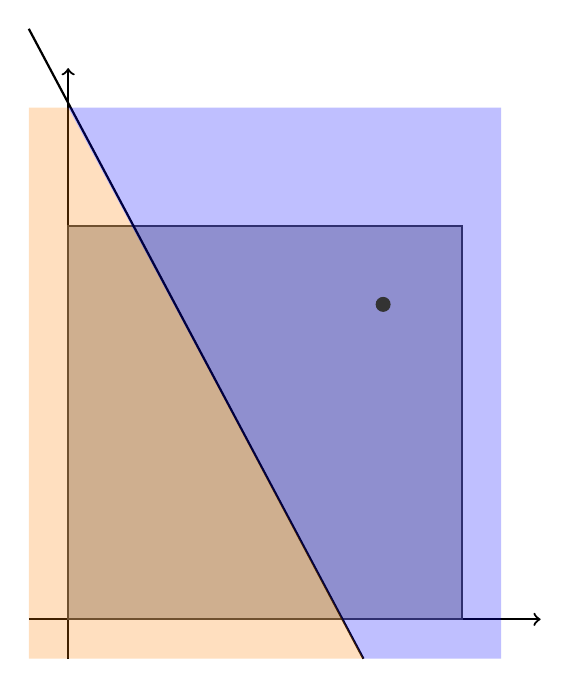
\begin{tikzpicture}[scale=5]
	\draw[black, thick, ->] (0, -0.1) -- (0, 1.4);  % y axis
	\draw[black, thick, ->] (-0.1, 0) -- (1.2, 0);  % x axis

	\filldraw[draw=black!75, fill=gray!50, thick] (0, 0) rectangle (1, 1);

	\draw[black, thick] (-0.1, 1.5) -- (0.75, -0.1);  % Boundary

	\fill[opacity=0.25, color=orange] (-0.1, -0.1) -- (-0.1, 1.3) -- (0, 1.3) -- (0.75, -0.1) -- cycle;
	\fill[opacity=0.25, color=blue] (0, 1.3) -- (0.75, -0.1) -- (1.1, -0.1) --  (1.1, 1.3) -- cycle;

	\filldraw[black!80] (0.8, 0.8) circle (0.5pt);

\end{tikzpicture}

% TODO: Add dotted lines indicating the point walking

% TODO: Add a second figure in which the point walks in both directions before hitting the boundary

% TODO: Put an alternative algorithm to do 1 step per variable, as opposed to discovering the range for 1 variable and then moving to the next one


\section{Experiments}

% TODO: Talk about that dataset $\{A \ge 0.5 \implies 1\}$ and mention how `anchor` fails to find the boundary (0.5)

% TODO: Talk about the execution time

% TODO: Talk about the correctness


\section{Conclusion}


\bibliographystyle{sbc}
\bibliography{sbc-template}

\end{document}
